\documentclass[18pt,a4paper]{extarticle}
\usepackage[utf8]{inputenc}
\usepackage{amsmath}
\usepackage{amsfonts}
\usepackage{amssymb}
\usepackage{graphicx}
\usepackage{booktabs}
\usepackage{listings}
\usepackage{siunitx}
\usepackage{url}
\usepackage
[
a4paper,% other options: a3paper, a5paper, etc
left=1cm,
right=1cm,
top=1cm,
bottom=1cm,
% use vmargin=2cm to make vertical margins equal to 2cm.
% us  hmargin=3cm to make horizontal margins equal to 3cm.
% use margin=3cm to make all margins  equal to 3cm.
]
{geometry}

\author{Frank Hermann}
\title{Comparison of Radar Stations for MSP Measurements}

\DeclareMathOperator{\sgn}{sgn}
\renewcommand{\d}[1]{\ensuremath{\operatorname{d}\!{#1}}}
\setlength\parindent{0pt}


\begin{document}
\begin{center}
	\textbf{\Large{A Simple Radar Code for the Low Altitude Ionosphere}}\\
	\small{Frank Hermann, 24.10.2021}
\end{center}
\pagenumbering{gobble}
\begin{figure}[h!]
	\centering
	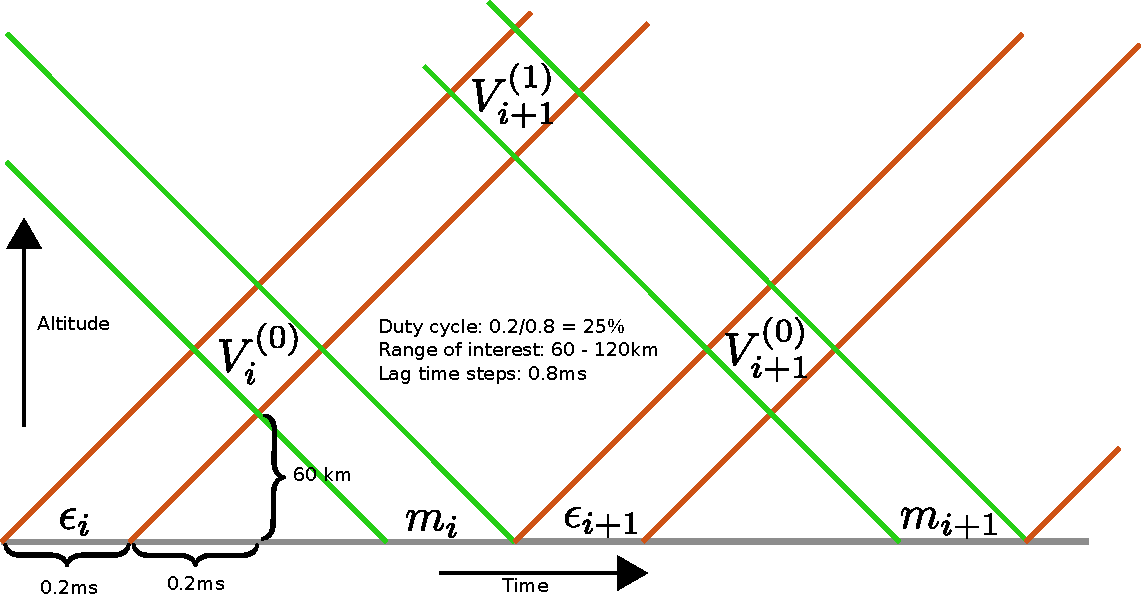
\includegraphics[width=0.9\linewidth]{code_diagram.pdf}
\end{figure}
We assume that the radar code $\epsilon$ is periodic $\epsilon_i = \epsilon_{i + L}$ and has already been transmitted for some time and that the radar continues transmitting the code indefinitely.
According to the sketch above, we see that
$$
\sum_{k=0}^{N-1} \epsilon_{i-k} V^{(k)}_i = m_i
$$
where $m_i$ is the $i$-th measured voltage and $N$ is the total number of range gates considered along the radar beam.
We calculate
\begin{align*}
\langle \epsilon_{j + \Delta}m_{j + \Delta + h}^* \epsilon_j^*m_{j+h}\rangle &= \epsilon_{j + \Delta}\epsilon_j^* \sum_{k=0}^{N-1} \epsilon_{j+\Delta+h-k}^*\epsilon_{j+h-k} \langle (V^{(k)}_{j + \Delta})^*V^{(k)}_j \rangle\\
&= \langle (V_{j+\Delta}^{(h)})^* V_j^{(h)} \rangle + \epsilon_{j + \Delta}\epsilon_j^*\sum_{k=0,k\neq h}^{N-1} \epsilon_{j+\Delta+h-k}^*\epsilon_{j+h-k} \langle (V^{(k)}_{j + \Delta})^*V^{(k)}_j \rangle
\end{align*}
where we have used the fact that signals from range gates of different altitudes do not correlate and assumed that $\epsilon_i^*\epsilon_i = 1$.
Furthermore, we have introduced $\Delta \in [1, M]$, where $M$ is the total number of measurement points in the auto correlation function.
Those will have the (desired) spacing of \SI{0.8}{\ms}.
The auto correlation function is defined as $\langle (V_{j+\Delta}^{(k)})^* V_j^{(k)} \rangle = R^{(k)}_\Delta$ assuming a wide sense stationary process for at least the time it takes to send the entire code once, which is $T = L\cdot\SI{0.8}{\ms}$.
We find for the auto correlation function at height $h$
$$
R^{(h)}_\Delta = \langle \epsilon_{j + \Delta}m_{j + \Delta + h}^* \epsilon_j^*m_{j+h}\rangle - \sum_{k=0, k\neq h}^{N-1} \epsilon_{j + \Delta}\epsilon_j^* \epsilon_{j+\Delta+h-k}^*\epsilon_{j+h-k} R_\Delta^{(k)}.
$$
In order to make the last term disappear we must average over the entire code to find the unbiased estimator
$$
\hat{R}^{(h)}_\Delta = \frac{1}{L}\sum^L_{j=1}\langle \epsilon_{j + \Delta}m_{j + \Delta + h}^* \epsilon_j^*m_{j + h}\rangle - \sum_{k=0, k \neq h}^{N-1}  R_\Delta^{(k)} \left[ \frac{1}{L} \sum^L_{j=0} \epsilon_{j + \Delta} \epsilon_j^*\epsilon_{j+\Delta+h-k}^*\epsilon_{j+h-k} \right]
$$
and demand that (with $W > w = k + H_1 - h + 1 > 0$ where $h \in [H_0, H_1]$ and $W=N+H_1 - H_0 + 1$)
$$
\frac{1}{L} \sum^L_{j=1} \epsilon_{j + \Delta} \epsilon_j^*\epsilon_{j+\Delta-w}^*\epsilon_{j-w} = 0.
$$
Due to technical limitations of the radar we have $\epsilon_i \in [-1, 1]$ and a naive brute force algorithm finds the following (shortest) codes for a given $W$ and $M$
\begin{center}
	\centering
	\begin{tabular}{cccc}
		\toprule
		$L$&$W$&$M$&Code\\
		\midrule
		24&5&4&$-+-+++++++-++--+-++-+++-$\\
		32&6&5&$-++-++++++++---++---+----++-+---$\\
		40&7&4&$-+--+++++++++-+++--+-+++----+-+++--++++-$\\
		\bottomrule
	\end{tabular}
\end{center}
Note that for $H_1 = H_0 = 0$ we can use that $k\neq h$ and find $W=N$.
\end{document}
